$subject$=Физические основы компьютерных \\ и сетевых технологий
$teacher$=Лекции Музыченко Я. Б.
$date$=02.12.2024

\section{12. Диполь. Электрическое поле в диэлектрике и проводнике.}

\Def Диполь - система из двух одинаковых по модулю разноименных точечных зарядов $+q$ и $-q$, 
находящихмя на расстоянии $l$ друг от друга.

Диполи в физике:

\begin{itemize}
    \item небольшие проводящие или диэлектрические тела в электрическом поле

    \item полярные молекулы
\end{itemize}

Электрический момент - основная характеристика диполя. Электрический момент - вектор $\vec{p} = q\vec{l}$, 
направленный от отрицательного заряда к положительного. Будем называть центром диполя середину вектора $l$ 

\ExN{1} Найдем потенциал поля в точке на оси диполя на расстоянии $r$ от центра диполя

$\varphi = \varphi_- + \varphi_+ = -\frac{kq}{r_-} + \frac{kq}{r_+} = kq \left(\frac{1}{r - \frac{l}{2}} - \frac{1}{r + \frac{l}{2}}\right) = 
\frac{kql}{r^2 - \frac{l^2}{4}}$

Так как $l \ll r$, $\varphi = \frac{kql}{r^2} = \frac{kp}{r^2}$

\ExN{2} Найдем потенциал поля в точке на перпендикуляре, проведенном через середину оси диполя, на расстоянии $r$ от центра

$\varphi = \varphi_- + \varphi_+ = -\frac{kq}{r_-} + \frac{kq}{r_+} = -\frac{kq}{r^\prime} + \frac{kq}{r^\prime} = 0$ - в силу симметрии

\ExN{3} В общем случае $\varphi = \frac{kp}{r^2} \cdot \cos\theta$, 
где $\cos\theta$ - острый угол между $l$ и радиус-вектором $r$ из центра диполя в точку

\begin{center}
    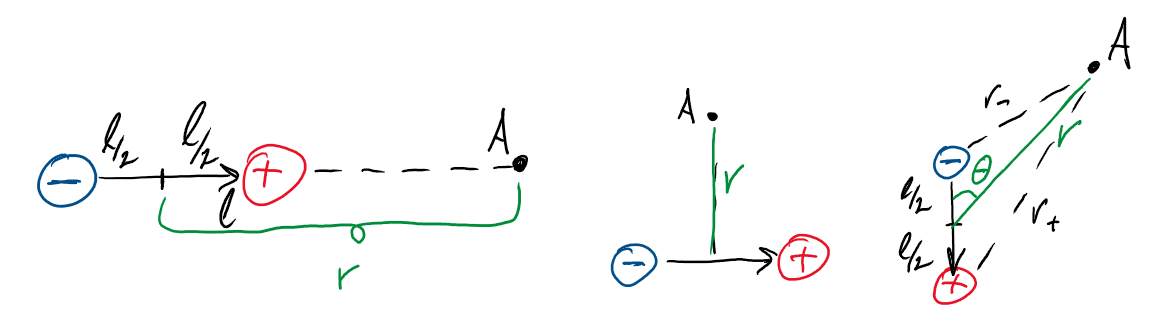
\includegraphics[width=0.8\textwidth]{physics1/images/physics1_2024_12_02_2}
\end{center}

\ExN{4} Найдем напряженность поля в точке на оси на расстоянии $r$

$E = E_- - E_+ = \frac{kq}{r_-^2} - \frac{kq}{r_+^2} = \frac{2kqrl}{(r - \frac{l}{2})^2 (r + \frac{l}{2})^2}$

При $l \ll r$ получаем $E = \frac{2kpr}{r^4} = \frac{2kp}{r^3}$


\ExN{5} Найдем напряженность поля в точке на перпендикуляре

По правилу суперпозиции вектор будет направлен влево

$\vec{E} = \vec{E}_+ + \vec{E}_-$

$E = 2E_+ \cos\alpha = \frac{2kq\cos\alpha}{r^2 + \frac{l^2}{4}} = \frac{2kq\frac{l}{2r_+}}{r^2 + \frac{l^2}{4}} \approx \frac{kp}{r^3}$

\ExN{6} В общем случае $E = \frac{kp}{r^3} \sqrt{1 + 3\cos^2 \theta}$

\begin{center}
    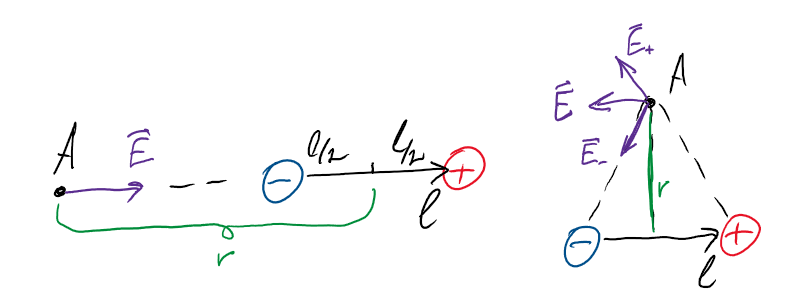
\includegraphics[width=0.8\textwidth]{physics1/images/physics1_2024_12_02_1}
\end{center}

\ExN{7} Если диполь поместить в однородное поле ($\vec{E} = \mathrm{const}$), то суммарная сила поля на заряды диполя равна 0.
Однако, если ось диполя расположена непараллельно линиям напряженности, то возникнет момент пары сил, заставляющий прийти диполь в устойчивое положение

\ExN{8} В неоднородном поле

$\vec{F} = \vec{F}_+ + \vec{F}_- = q(\vec{E}_- + \vec{E}_+) = q\Delta\vec{E}$

$\Delta\vec{E} = \frac{\Delta\vec{E}l}{l} = \frac{\partial \vec{E}}{\partial l}l \Longrightarrow \vec{F} = p\frac{\partial \vec{E}}{\partial l}$

Найдем момент сил, действующих на диполь в неоднородном поле:

$\vec{F}_+ = q\vec{E}_+ \quad \vec{F}_- = q\vec{E}_- \ (|\vec{E}_+| = |\vec{E}_-|)$

$\vec{M} = \vec{M}_1 + \vec{M}_2 = [\vec{r}_+ \vec{F}_+] + [\vec{r}_- \vec{F}_-] = [\vec{r}_+ \vec{F}_+] - [\vec{r}_- \vec{F}_+] = 
[\vec{r}_+ - \vec{r}_-, q\vec{E}] = [\vec{l}, q\vec{E}] = [\vec{p}\vec{E}]$

$\vec{M} = [\vec{p}\vec{E}]$

Если $\vec{p} \uparrow\uparrow \vec{E}, \vec{M} = 0$ - устойчивое положение равновесия

Если $\vec{p} \uparrow\downarrow \vec{E}, \vec{M} = 0$ - неустойчивое положение

\begin{center}
    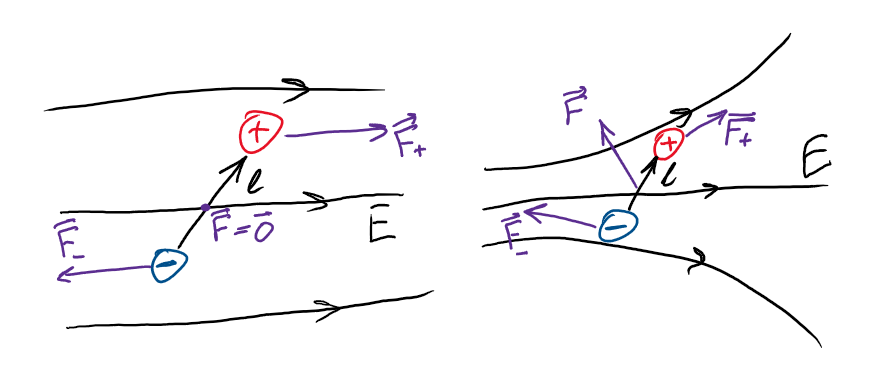
\includegraphics[width=0.8\textwidth]{physics1/images/physics1_2024_12_02_3}
\end{center}


Энергия пары зарядов в поле

$W = q \varphi_+ - q\varphi_- = q\Delta\varphi \qquad W = q\frac{\partial \varphi}{\partial l}l$

Получаем $\frac{\partial \varphi}{\partial l} = -E_l$

\Def Проводники - тела, в которых имеются свободные заряды, способные свободно перемещаться внутри этих тел, следовательно,
проводящие точке

\Def Диэлектрики-изоляторы - вещества, практически не проводящие электрического тока. В диэлектрике нет 
свободных зарядов, способных перемещаться на значительные расстояния

\Def Полярные молекулы - молекулы, у которых центр \enquote{тяжести} отрицательного заряда сдвинут относительно положительного. 
В отсутствие внешнего электрического поля обладают собственным дипольным моментом

\Def Неполярные молекулы - молекулы, у которых центры положительного и отрицательного зарядов совпадают

\Def Поляризация - физический процесс пространственного разделения зарядо под действием внешнего электрического поля

При внесении неполярного диэлектрика во внешнее электрическое поля внутри каждой молекулы происходит смещение зарядов

В полярном диэлектрике диполи направлены хаотично, поэтому их сумма приблизительно равна нулю. 
При внесении полярного диэлектрика происходит ориекнтация дипольных моментов по направлению поля

На поверхности диэлектрика в результате поляризации появляются связанные (поляризационные) заряды. Обозначаются 
$q_\text{связ}, \sigma_\text{связ}, q^\prime, \sigma^\prime$

Свободные (сторонние) заряды - заряды, которые под действием внешнего поля могут перемещаться по всему объему 
вещества. Такие заряды по определению не содержатся в диэлектриках. 
Обозначаются $q_\text{своб}, \sigma_\text{своб}, q^\prime, \sigma^\prime$
